\documentclass{standalone}
\usepackage{tikz}
\usetikzlibrary{shapes.geometric, arrows, positioning, calc}

\begin{document}
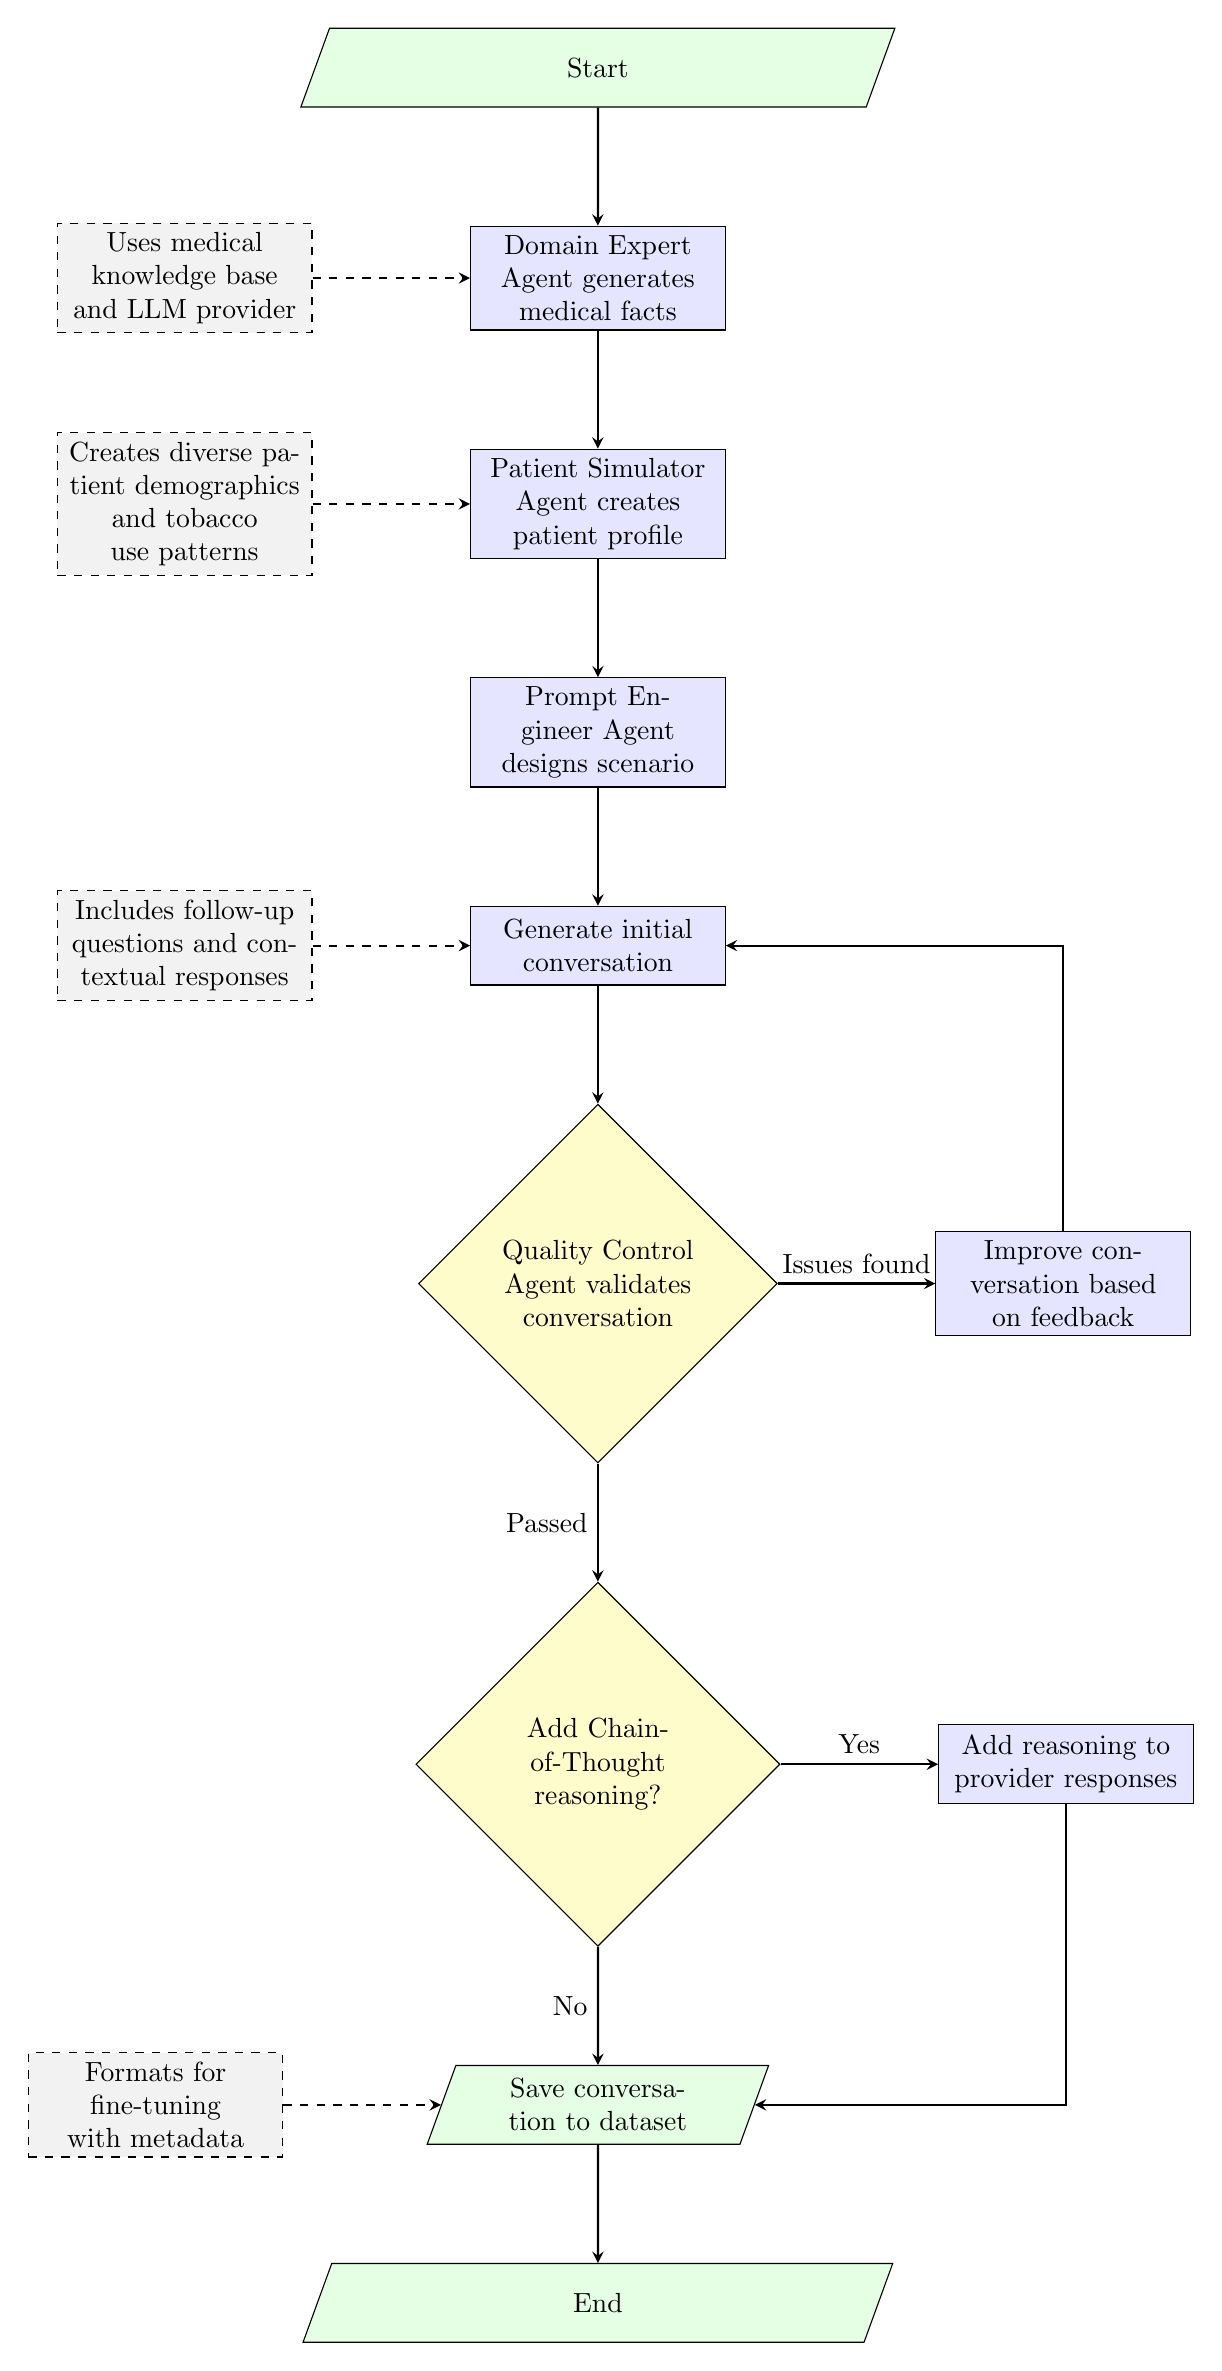
\begin{tikzpicture}[
    node distance=1.5cm,
    process/.style={rectangle, draw, text width=3cm, text centered, minimum height=1cm, fill=blue!10},
    decision/.style={diamond, draw, text width=3cm, text centered, minimum height=1cm, fill=yellow!20},
    io/.style={trapezium, trapezium left angle=70, trapezium right angle=110, draw, text width=3cm, text centered, minimum height=1cm, fill=green!10},
    arrow/.style={thick,->,>=stealth},
    note/.style={rectangle, draw, dashed, text width=3cm, text centered, minimum height=1cm, fill=gray!10}
]

% Start
\node[io] (start) {Start};

% Domain Expert Agent
\node[process, below=of start] (domain) {Domain Expert Agent generates medical facts};

% Patient Simulator Agent
\node[process, below=of domain] (patient) {Patient Simulator Agent creates patient profile};

% Prompt Engineer Agent
\node[process, below=of patient] (prompt) {Prompt Engineer Agent designs scenario};

% Generate Conversation
\node[process, below=of prompt] (generate) {Generate initial conversation};

% Quality Check
\node[decision, below=of generate] (quality) {Quality Control Agent validates conversation};

% Improve Conversation
\node[process, right=2cm of quality] (improve) {Improve conversation based on feedback};

% Chain of Thought
\node[decision, below=of quality] (cot) {Add Chain-of-Thought reasoning?};

% Add CoT
\node[process, right=2cm of cot] (addcot) {Add reasoning to provider responses};

% Save Conversation
\node[io, below=of cot] (save) {Save conversation to dataset};

% End
\node[io, below=of save] (end) {End};

% Notes
\node[note, left=2cm of domain] (note1) {Uses medical knowledge base and LLM provider};
\node[note, left=2cm of patient] (note2) {Creates diverse patient demographics and tobacco use patterns};
\node[note, left=2cm of generate] (note3) {Includes follow-up questions and contextual responses};
\node[note, left=2cm of save] (note4) {Formats for fine-tuning with metadata};

% Arrows
\draw[arrow] (start) -- (domain);
\draw[arrow] (domain) -- (patient);
\draw[arrow] (patient) -- (prompt);
\draw[arrow] (prompt) -- (generate);
\draw[arrow] (generate) -- (quality);
\draw[arrow] (quality) -- node[above] {Issues found} (improve);
\draw[arrow] (improve) |- (generate);
\draw[arrow] (quality) -- node[left] {Passed} (cot);
\draw[arrow] (cot) -- node[above] {Yes} (addcot);
\draw[arrow] (addcot) |- (save);
\draw[arrow] (cot) -- node[left] {No} (save);
\draw[arrow] (save) -- (end);

% Note connections
\draw[arrow, dashed] (note1) -- (domain);
\draw[arrow, dashed] (note2) -- (patient);
\draw[arrow, dashed] (note3) -- (generate);
\draw[arrow, dashed] (note4) -- (save);

\end{tikzpicture}
\end{document}
